% Nikolai Nielsens "Fysiske Fag" preamble
\documentclass[a4paper,10pt]{article} 	% A4 papir, 10pt størrelse
\usepackage[english]{babel}
\usepackage{Nikolai} 					% Min hjemmelavede pakke
\usepackage[dvipsnames]{xcolor}
\usepackage{gensymb}

% Margen
\usepackage[margin=1in]{geometry}

% Max antal kolonner i en matrix. Default er 10
%\setcounter{MaxMatrixCols}{20}

% Hvor dybt skal kapitler labeles?
%\setcounter{secnumdepth}{4}	
%\setcounter{tocdepth}{4}


% Hvilket nummer skal der startes med i sections? (n-1)
%\setcounter{section}{0}	

% Til nummerering af ligninger. Så der står (afsnit.ligning) og ikke bare (ligning)
\numberwithin{equation}{section}


% Header
%\usepackage{fancyhdr}
%\head{}
%\pagestyle{fancy}

%Titel
\title{Numerical Methods in Physics Week 1}
\author{Nikolai Plambech Nielsen}
\date{}

\begin{document}
	\maketitle
	\section{Nuclear Decay}
	Suppose  two radioactive isotopes, A and B, are present with populations $ N_A(t) $ and $ N_B(t) $, and decay times $ \tau_A $  and $ \tau_B $. Type A decays into type B, while B decays into something not tracked. The relevant differential equations are
	\begin{equation}
		\diff[\ud]{N_A}{t} = - \frac{N_A}{\tau_A}, \quad \diff[\ud]{N_B}{t} = \frac{N_A}{\tau_A} - \frac{N_B}{\tau_B}.
	\end{equation}
	The purpose of this assignment is to solve this problem numerically for a number of different conditions, using Euler integration. This method is used for its simplicity and ease of implementation. For all of the following simulations and plots, the value $ \Delta t = 0.1 $ is used.
	
	\subsection{Compare the numerical and analytical solutions}
	The analytical solutions are given in the assignment, and are as follows:
	\begin{align}
		N_A(t) &= N_A(0) \exp\pp{-\frac{t}{\tau_A}}, \\
		N_B(t) &= \begin{cases}
		N_B(0) \exp\pp{-\frac{t}{\tau_A}} + t \frac{N_A(0)}{\tau_A} \exp\pp{-\frac{t}{\tau_A}}, & \tau_A= \tau_B, \\
		N_B(0) \exp\pp{-\frac{t}{\tau_B}} + \frac{N_A(0)}{\frac{\tau_A}{\tau_B} - 1} \bb{\exp\pp{-\frac{t}{\tau_A}} - \exp\pp{-\frac{t}{\tau_B}}}, & \tau_A \neq \tau_B.
		\end{cases}
	\end{align}	
	The results, along with residual plots, for $ N_A(0) = N_B(0) = 1000 $ and $ \tau_A = 5, \tau_B = 10 $ are shown below, with the analytical solution for $ \tau_A \neq \tau_B $:
	\begin{figure}[H]
		\centering
		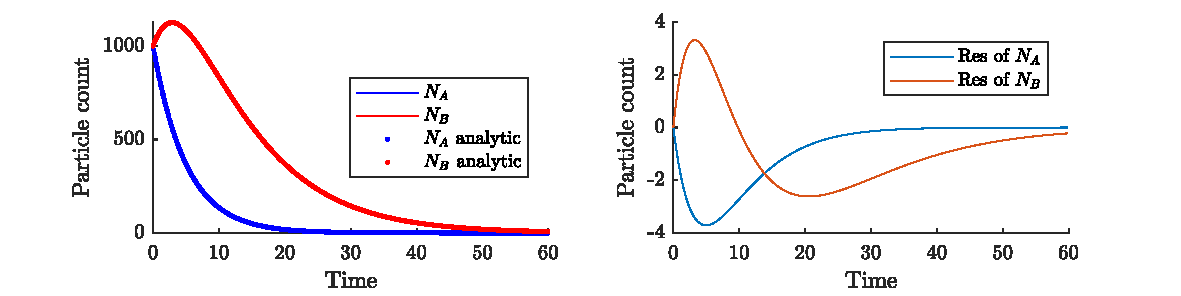
\includegraphics[width=\linewidth]{unequaltau.pdf}
		\caption{Two plots of nuclear decay as a function of time. In the left plot, the numerical and analytical solutions are shown on the same plot, while in the right plot, the residuals of $ N_A $ and $ N_B $ are shown to highlight the discrepancy between the analytical and numerical solutions to the problem.}
		\label{fig:unequalTau}
	\end{figure}
	To demonstrate the solution for $ \tau_A = \tau_B $, the initial conditions of $ N_A=N_B = 1000 $ and $ \tau_A=\tau_B = 10 $ are shown below. Again with accompanying residual plots:
	\begin{figure}[H]
		\centering
		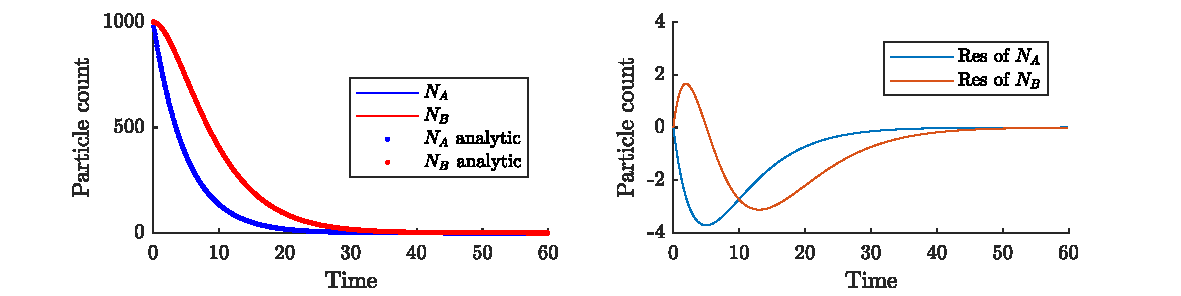
\includegraphics[width=\linewidth]{equaltau.pdf}
		\caption{Same plot setup as in figure \ref{fig:unequalTau}, but with equal values for $ \tau_A $ and $ \tau_B $.}
		\label{fig:equalTau}
	\end{figure}
	As seen in both figures \ref{fig:unequalTau} and \ref{fig:equalTau}, the numerical is close to the analytical solution, differing by less than 4 at all times, for each of the cases. An increase in $ N_B $ is seen in figure \ref{fig:unequalTau} due to the faster decay of type A than that of type B.
 	
	\subsection{Explain the limit of $ \tau_A/\tau_B \gg 1 $}
	In this limit, the decay of type $ B $ is much faster than that of type $ A $. This means, that on any appreciable time scale of change for $ N_A $, the population of $ B $ reaches a steady-state solution, where $ \ud N_B/\ud t = 0 $. As such the differential equation for $ N_B $ becomes
	\begin{equation}\label{eq:steadyNB}
		\diff[\ud]{N_B}{t} = \frac{N_A}{\tau_A} - \frac{N_B}{\tau_B} = 0, \quad \Rightarrow \quad N_B(t) = N_A \frac{\tau_B}{\tau_A}.
	\end{equation}
	This is also seen in a simulation, where $ \tau_A = 3600,\tau_B = 5 $:
	\begin{figure}[H]
		\centering
		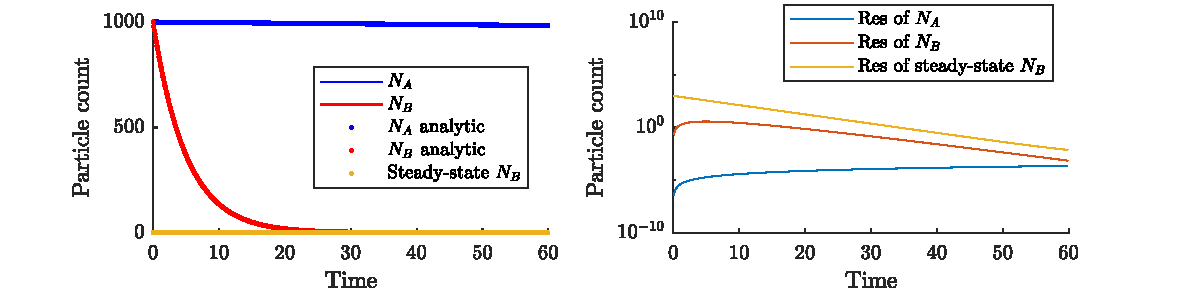
\includegraphics[width=\linewidth]{largetau.pdf}
		\caption{Plot of the numerical and analytical solutions to the decay problem (left) and associated residuals (right). In both cases, the steady-state solution for $ N_B $ is also plotted.}
		\label{fig:largeTau}
	\end{figure}
	as seen, the steady-state solution for $ N_B $ (\eqref{eq:steadyNB}) does correctly predict the behaviour for $ N_B $, when this is approximately 0. This makes sense; the change in $ N_A $ is almost constant, corresponding to when $ N_B $ is approximately 0, which is the steady state for this particular problem.
	
	
	\section{Projectile motion}
	For this assignment, projectile motion is to be simulated, again using the Euler-method. This gives another example of how to use this simple method of simulation, for a problem which (without wind resistance) has an analytical solution. After this, uncharted waters are encountered, when wind resistance is included. Here no analytical solution is given, and all reliance upon the previous methods, like residuals between the numerical and analytical solutions, are not applicable.
	
	Furthermore, for this problem, a second derivative is used, whereby a second Euler integration is needed, to complete the time step. The relevant differential equations are
	\begin{equation}
		\diff[\ud]{\V{r}}{t} = \V{v}, \quad \diff[\ud]{\V{v}}{t} = -g\Vy.
	\end{equation}
	where the analytical solution is computed by integrating the second equation twice, and using the relevant initial conditions:
	\begin{equation}
		\V{r}(t) = \begin{pmatrix}
		x(t) \\ y(t)
		\end{pmatrix} = \begin{pmatrix}
		x_0+v_{x,0} t \\ y_0+v_{y,0}t-gt^2/2
		\end{pmatrix}. 
	\end{equation}
	
	
	\subsection{Without wind resistance}
	The numerical and analytical solutions to projectile motion, given the initial conditions of $ x_0 = 0,y_0 = 2 \e{m},v_0 = 4 \e{m/s}$ and $ \theta = 70\degree$, where $ v_{x,0} = v_0 \cos \theta $ and $ v_{y,0} = v_0 \sin \theta $. For the numerical solution a value of $ \Delta t = 0.01 \e{s}$ is used. The results are shown below, along with the absolute residual, as a function of time:
	\begin{figure}[H]
		\centering
		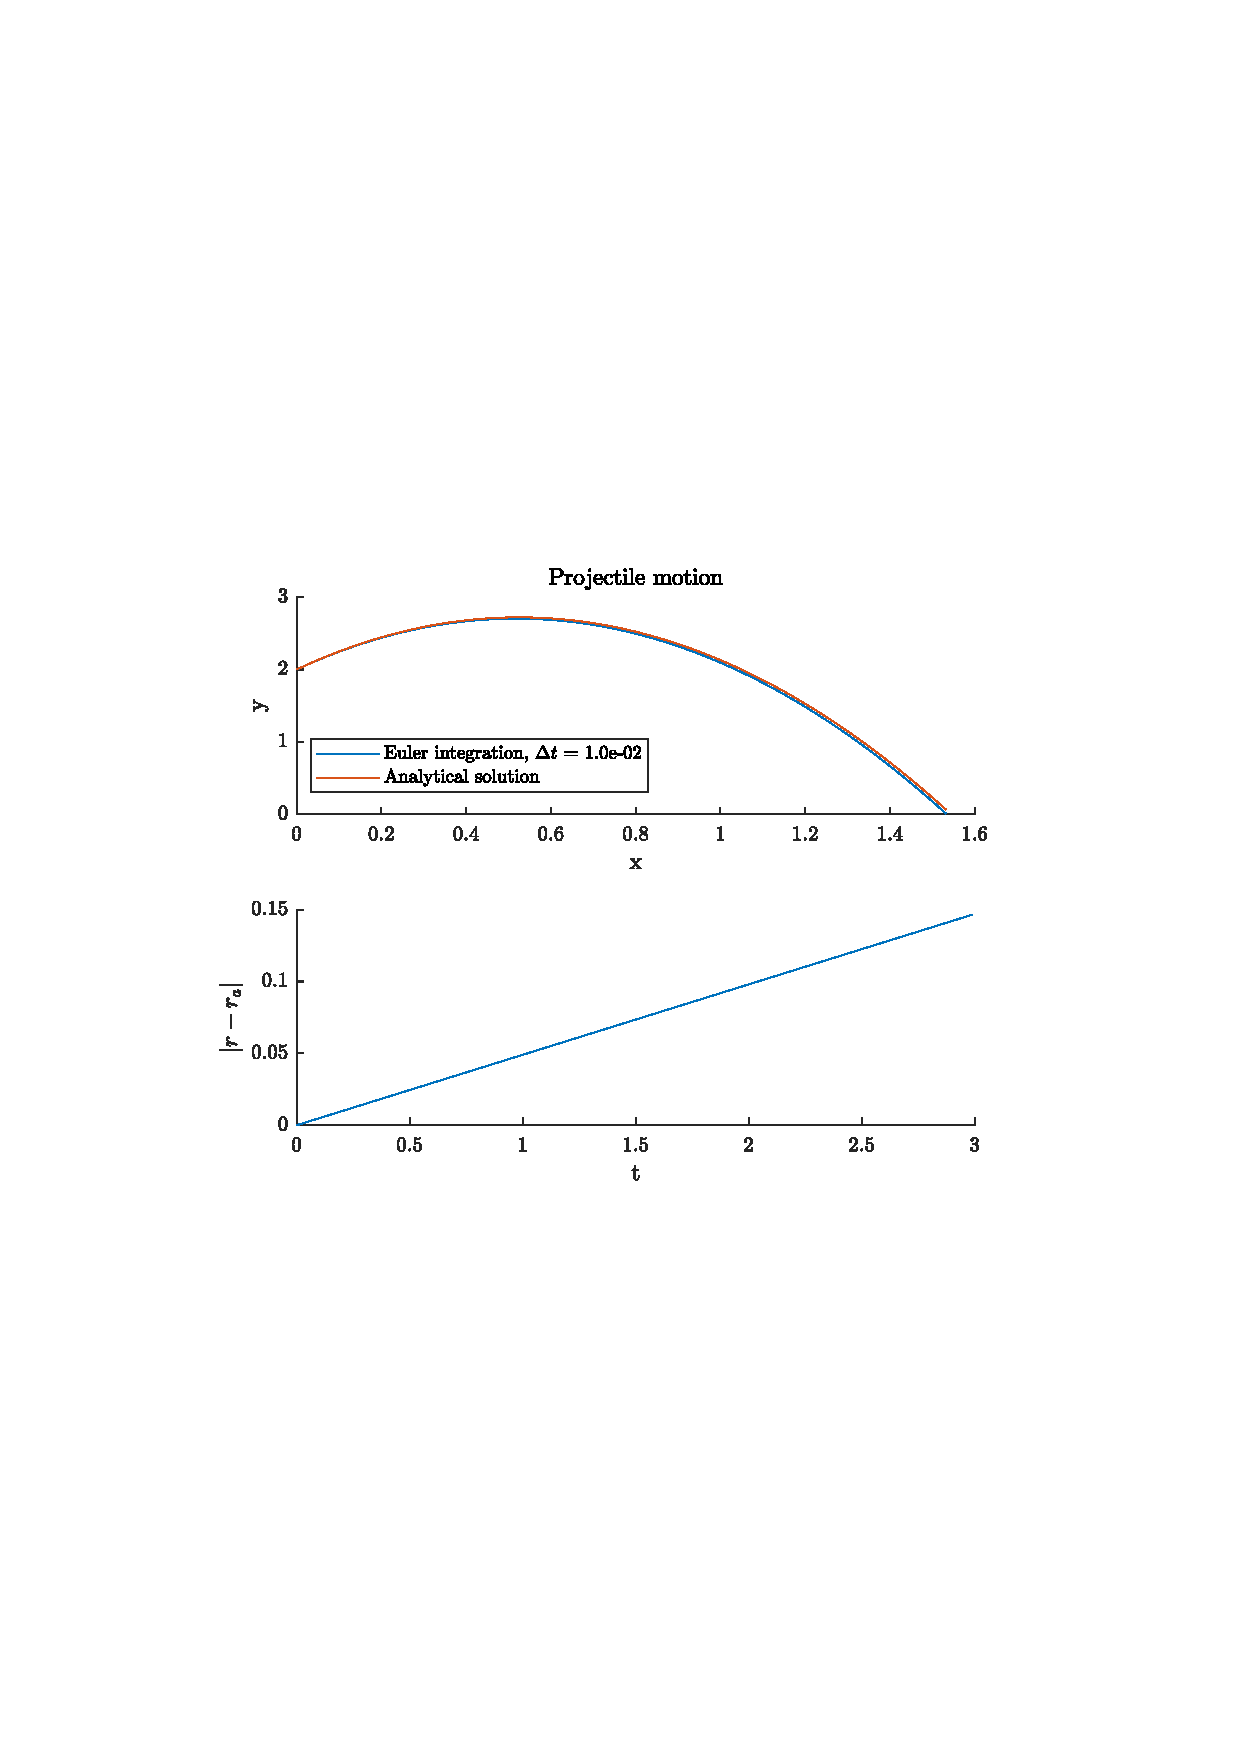
\includegraphics[width=\linewidth]{projectile.pdf}
		\caption{Plots of the numerical and analytical solutions to projectile motion (left) and the absolute residual (right).}
		\label{fig:projectile}
	\end{figure}
	the absolute residual is also the global truncation error, as defined in the slides for the week 1 lectures. As is expected, the error increases linearly in time, given the linear increase in velocity. This means that the Euler integration underestimates the velocity by a constant amount per time step, leading to a linear increase in global truncation error.
	
	
	Next the effect of the size of the time step $ \Delta t $ is analysed. This is done by creating a vector of logarithmically spaced values for $ \Delta t $, between $ 10^{-1} \e{s} $ and $ 10^{-8} \e{s}$, running the simulation, and recording the global truncation error. If any smaller step size is to be investigated, the simulation as to be broken into pieces, as the size of the arrays exceed the amount of memory available on the desktop workstation used.
	
	This could be done by recording the first, say, $ 10^6 $ steps, storing the final results, clearing the arrays from memory and then running the simulation again, with the final results as the new initial conditions, until the full simulation has been completed.
	
	However, with the step sizes as mentioned, the final global truncation error becomes
	\begin{figure}[H]
		\centering
		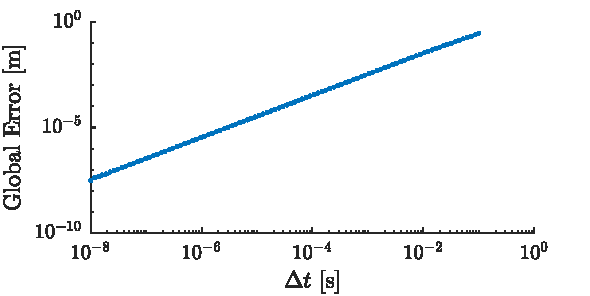
\includegraphics[width=0.5\linewidth]{projError.pdf}
		\caption{A plot of the global error of the simulation, as a function of the time step size $ \Delta t $.}
		\label{fig:projError}
	\end{figure}
	On the double-log plot, the relation between global truncation error and time step size is definitely polynomial, as the graph is that of a straight line. The slope then corresponds to the polynomial degree, and as this is approximately 1, the relation is taken as being linear.
	
	\subsection{With wind resistance}
	Next a drag force, quadratic in velocity, is introduced to the problem. The formula is
	\begin{equation}
		\V{F}_d = -\frac{1}{2}C_D \rho A v \V{v}
 	\end{equation} 
 	where $ C_D $ is the coefficient of drag for the projectile, $ \rho $ is the density of the surrounding media, $ A $ is the cross sectional area of the projectile, and $ v $ is the magnitude of the velocity vector $ \V{v} $. As seen, this is directed opposite to the velocity. The differential equations become:
 	\begin{equation}
 			\diff[\ud]{\V{r}}{t} = \V{v}, \quad \diff[\ud]{\V{v}}{t} = -\frac{1}{2m}C_D \rho A v \V{v} -g\Vy.
 	\end{equation}
 	where now the second differential equation is no longer linear, owing to the quadratic term in velocity.
 	
 	With no analytical solution given, other means for estimating the error has to be utilized. As confirmed in the example with no wind resistance, the global truncation error is linearly related to the size of the time step $ \Delta t $. As such, the global truncation error on the simulation with wind resistance will also approach 0 as the size of $ \Delta t $ is decreased. Given this, a method of attaining a desired level of precision is needed.
 	
 	For the problem at hand, the simulation is run with 100 logarithmically spaced values between $ 10^{-1} \e{s}$ and $ 10^{-8} \e{s} $. The final point of impact is logged, along with the time taken to run the simulation. The results are shown below on semilog and double-log plots respectively:
 	\begin{figure}[H]
 		\centering
 		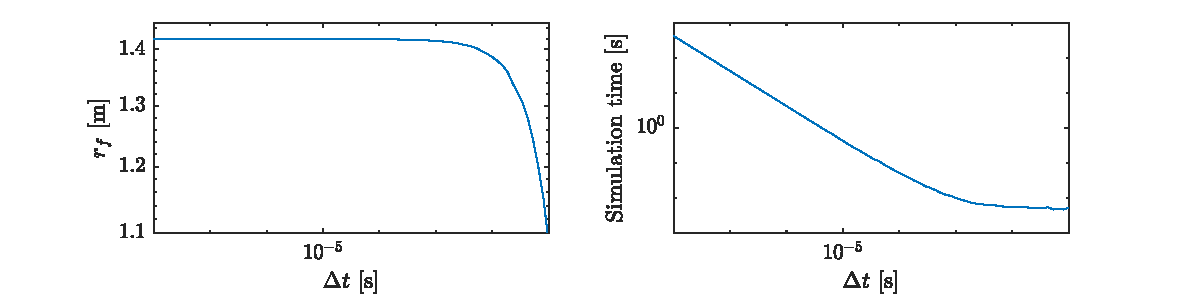
\includegraphics[width = \linewidth]{simtime.pdf}
 		\caption{Semilog plot of the final distance (left) and double-log plot of the simulation time (right). Both as a function of $ \Delta t $.}
 		\label{fig:simtime}
 	\end{figure}
 	The reason for also recording the simulation time is that while a simulation taking a week to run might be the most precise result achievable, it is not very practical, and might not be that much more precise than that of a simulation that only takes a minute or two. For example, the final simulation, with $ \Delta t = 10^{-8} \e{s} $, took just under 7 minutes. The simulation with the smallest $ \Delta t $, coming within 1\% of the result of the final simulation took just 0.0061 seconds, with a time step size of $ \Delta t = 0.0043 s $. So while the precision is within 1 \% of the final simulation, the run time is almost 5 orders of magnitude smaller. The desired precision can of course be chosen as needed, achieving a precise enough results whilst keeping run time small enough to be practical.
 	
 	
 	\section{Orbits of comets}
 	For this assignment, the trajectory of particles in a gravitational field is calculated both using Euler integration and 4th order Runge-Kutta integration (RK4), which uses a weighted average of several derivatives with smaller time steps, to calculate the final value of the next time step. The differential equations for this problem is
 	\begin{equation}
 		\diff[\ud]{\V{r}}{t} = \V{v}, \quad \diff[\ud]{\V{v}}{t} = \frac{GM}{r^2}\U{r} = \frac{GM}{r^3}\V{r},
 	\end{equation}
 	where, for the purpose of simplicity, $ GM $ is set to $ 4\pi^2 \e{(AU)}^3/\e{(yr)}^3 $. This gives a circular orbit for an initial radius of $ 1 \e{AU} $ and initial tangential velocity of $ 2 \pi \e{AU}/\e{yr} $. Furthermore, the mass of the comet in orbit, is set to unity. 
 	
 	\subsection{Euler and RK4}
 	First, the two methods are compared for a circular orbit with a step size of $ \Delta t = 0.02 \e{yr} $ and a total simulation time of $ 1 \e{yr} $. The trajectories are shown in the figure below:
 	
	\begin{figure}[H]
		\centering
		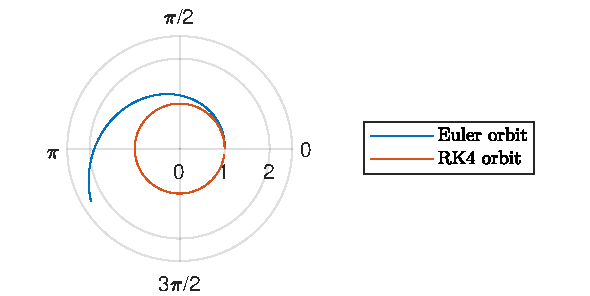
\includegraphics[width=0.7\linewidth]{CircOrbit.pdf}
		\caption{Simulation of a circular orbit using both the Euler method and the 4th order Runge-Kutta method.}
		\label{fig:CircOrbit}
	\end{figure}
 	As seen, neither of the simulations actually complete an orbit, however the Runge-Kutta method comes significantly closer. To quantify this, the following fractional error is calculated:
 	\begin{equation}
 		\text{err} = \frac{|\V{r}_f-\V{r}_0|}{|\V{r}_0|}
 	\end{equation}
 	where $ \V{r}_0 $ is the initial and $ \V{r}_f $ is the final position of the comet. Next, the simulation is run for 60 different values of $ \Delta t $, logarithmically spaced between $ 10^{-1} \e{yr} $ and $ 10^{-6} \e{yr} $:
	\begin{figure}[H]
		\centering
		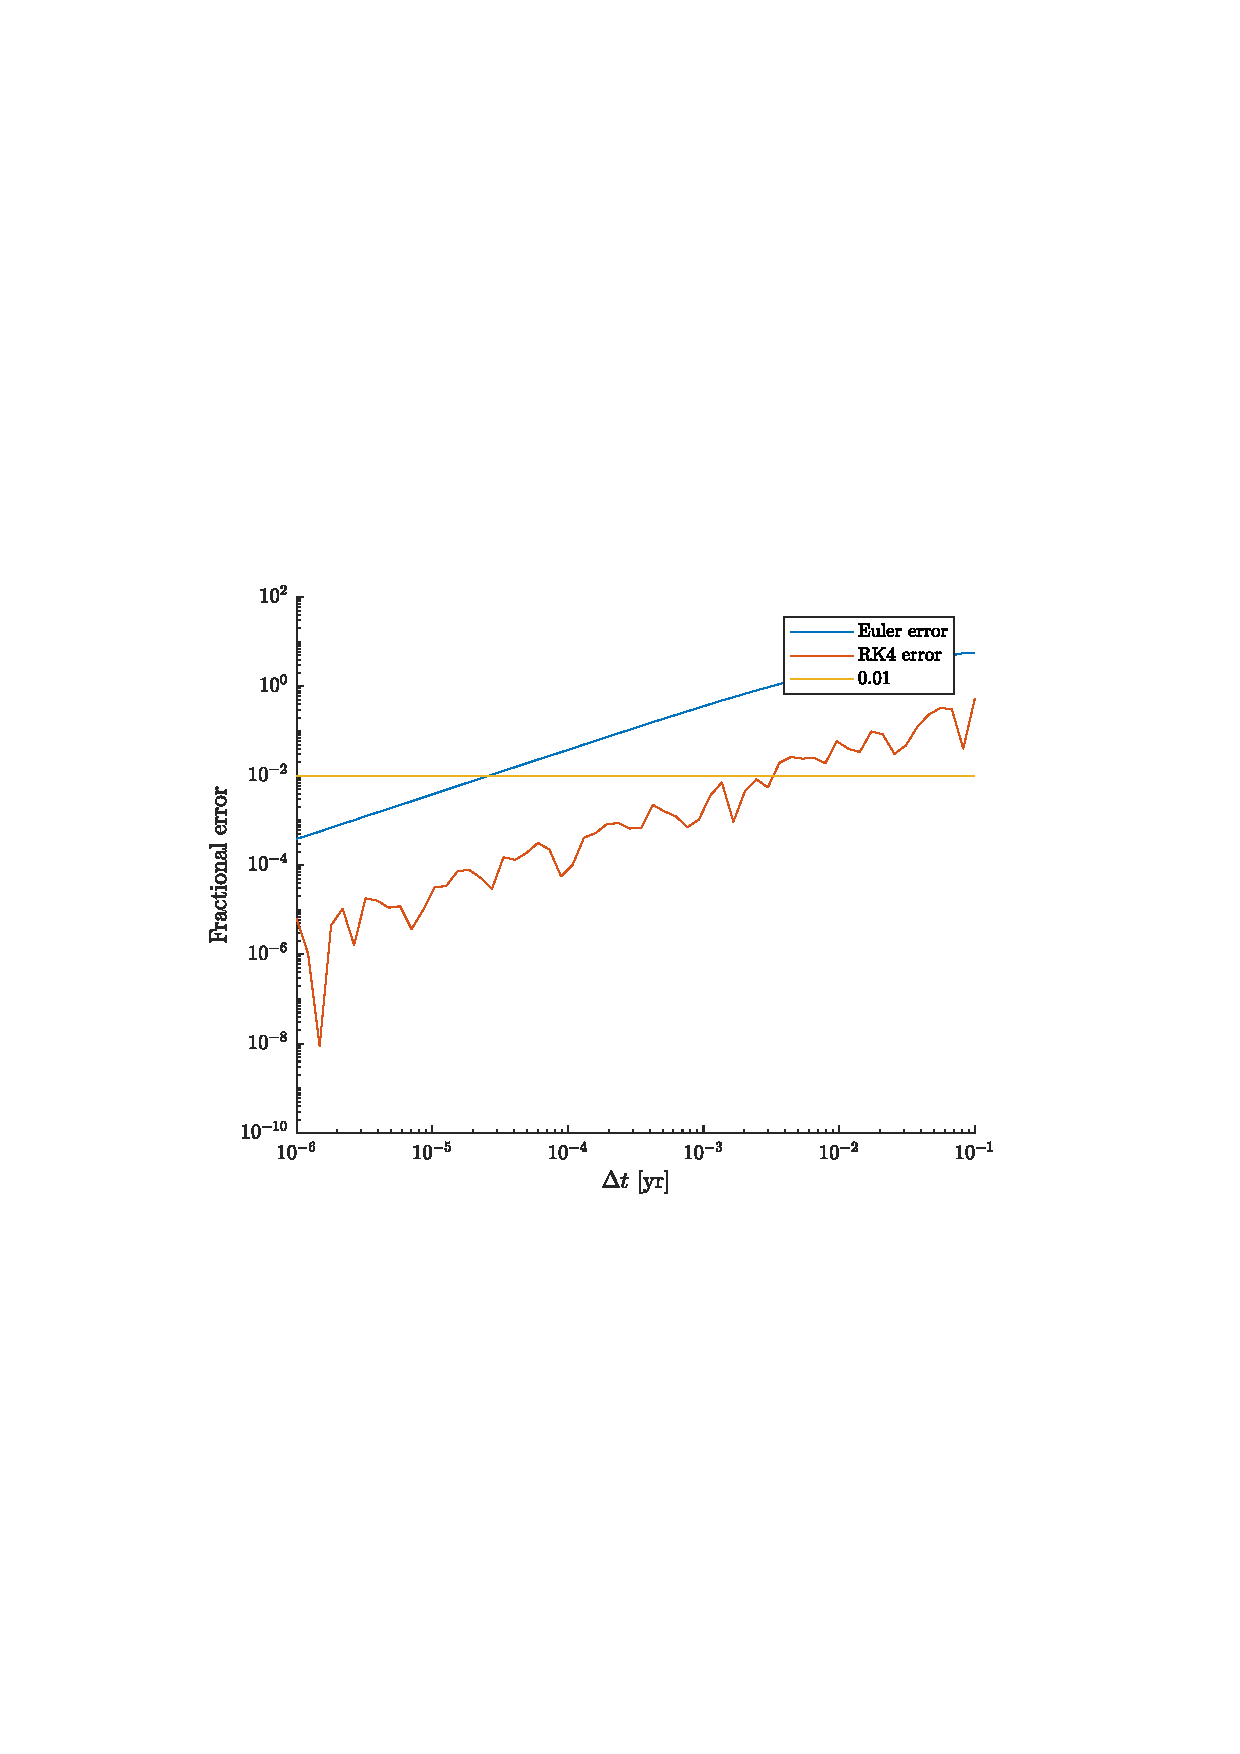
\includegraphics[width=0.8\linewidth]{KeplerdtErr.pdf}
		\caption{A plot of the global fractional error as a function of the time step size $ \Delta t $, for both the Euler and Runge-Kutta methods. A horizontal line for 1\% is included for clarity.}
		\label{fig:KeplerdtErr}
	\end{figure}
	As seen from the figure, the Runge-Kutta method consistently outperforms the Euler method in fractional error, though the error in the Runge-Kutta method fluctuates, sometimes over an order of magnitude. Rounded up, the Runge-Kutta needs a $ \Delta t $ of the order $ 10^{-3} \e{yr} $ to have a fractional error lower than 1\%, whilst the Euler method needs one in the order of $ 10^{-5} \e{yr} $, 2 orders of magnitude lower.
	
	\subsection{RK4 and the analytical solution}
	For this problem, the analytical solution is also known, and the radius, as a function of the angle $ \theta $, is given by
	\begin{equation}
		r(\theta) = \frac{a(1-\epsilon^2)}{1-\epsilon \cos \theta}
	\end{equation}
	where $ \epsilon = \sqrt{1-b^2/a^2}$ is the eccentricity of the orbit, $ a $ is the semimajor axis and $ b $ is the semiminor axis of the orbit. The semimajor and semiminor axes are given respectivle by the arithmetic and geometric mean of the largest and smallest radius:
	\begin{equation}
		a = \frac{r_{\text{max}}+r_{\text{min}}}{2}, \quad b = \sqrt{r_{\text{max}r_{\text{min}}}}.
	\end{equation}
	Next the Runge-Kutta method is compared to the analytical solution. The smallest and largest radii of the orbit are calculated after the full simulation has run, and the magnitude of the radius is calculated at each point along the orbit. To compare the two solutions, two initial conditions are chosen: both starting at a radial distance of $ 1 \e{AU} $, with initial tangential velocity of $ \pi \e{AU/yr} $ and $ 2 \pi \e{AU/yr} $. Both simulations are run with a step size of $ \Delta t  = 0.005 \e{yr} $.
	
	The simulation uses cartesian coordinates, so to retrieve the angle used in the analytical solution the function \texttt{atan2} is used. This is different to the normal arctangent function in that \texttt{atan2} takes two inputs, $ y $ and $ x $, whereas the normal arctangent only takes one $ v = y/x $. The normal arctangent function is only defined for angles between $ -\pi/2 $ and $ \pi/2 $ radians, so in the right half-plane. But the \texttt{atan2} function works for all angles between $ 0 $ and $ 2\pi $ radians, and as such is the one needed for this problem.
	
	With the angle, semimajor and semiminor axes calculated, the analytical solution can be computed. The numerical solution is then compared by computing the absolute fractional error across the entire period of an orbit:
	\begin{equation}
		\text{err} = \vv{\frac{r_{\text{numerical}}-r_{\text{analytical}}}{r_{\text{analytical}}}}
	\end{equation}
	The results, for the two initial conditions are shown in the figures below:
	\begin{figure}[H]
		\centering
		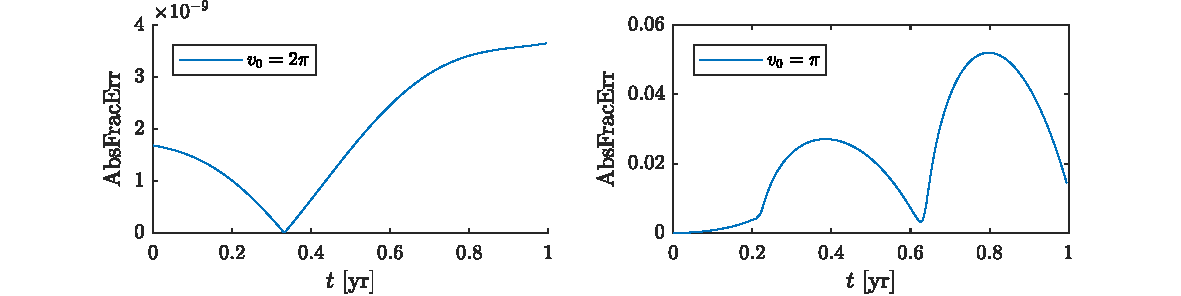
\includegraphics[width = \linewidth]{KeplerFracErr.pdf}
		\caption{Plots of the absolute fractional error between the analytical and numerical solution to the Kepler problem. On the left for a circular orbit and on the right for an elliptical orbit.}
		\label{fig:KeplerAnalytical}
	\end{figure}
	For the circular orbit the absolute fractional error is exceedingly small, 9 orders of magnitude below unity, whilst for the elliptical orbit it is in the small percentages, between 0 and 6 percent. The reason for the dips in fractional error is seen in figure \ref{fig:KeplerAdaptive2}, as the Runge-Kutta method slowly circles inwards but at the smallest radius, the orbits align again.

	\subsection{Adaptive 4th order Runge-Kutta}
	For this last exercise, an adaptive version of the 4th order Runge-Kutta method is introduced. This performs the integration three times. Once normally, and then twice in a row, with half the time step size, to get one full integration with the chosen step size. The big step is called $ x_b(t+\Delta t) $ and the result of the small step(s) is called $ x_s(t_+\Delta t) $. If the error, defined as $ \text{err} = |x_b(t+\Delta t)-x_s(t+\Delta t) |$, is smaller than some specified upper bound, the time step size $ \Delta t $ is accepted and increased for the next time step, but if the error is \textit{larger} than the upper bound, the step size is rejected, decreased, and the error is calculated again with the smaller step size.
	
	This allows the simulation to have a starting size for $ \Delta t $, but to increase it when the function is only changing slowly, and decreasing it when the function is changing rapidly. 
	
	For the same initial conditions as before, when comparing the analytical and regular Runge-Kutta method, the adaptive and non-adaptive Runge-Kutta methods are compared, by calculating the trajectories and evolution of energy, as a function of time.
	\begin{figure}[H]
		\centering
		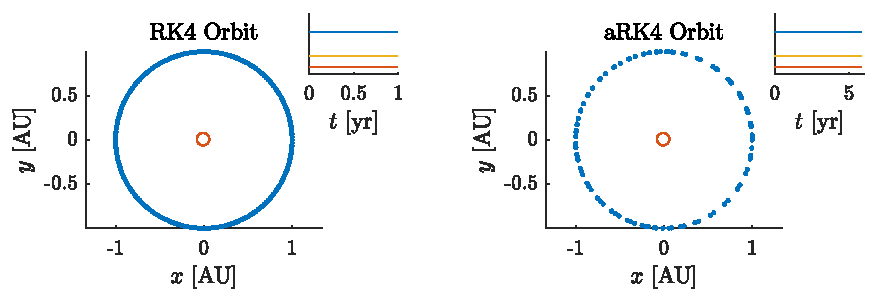
\includegraphics[width = \linewidth]{RK42pi.pdf}
		\caption{Plots of the trajectory of a circular orbit, along with inset plots of the kinetic (blue), potential (red), and total energy (orange), as a function of time, for the Runge-Kutta (left) and adaptive Runge-Kutta (right) methods.}
		\label{fig:KeplerAdaptive1}
	\end{figure}
	\begin{figure}[H]
		\centering
		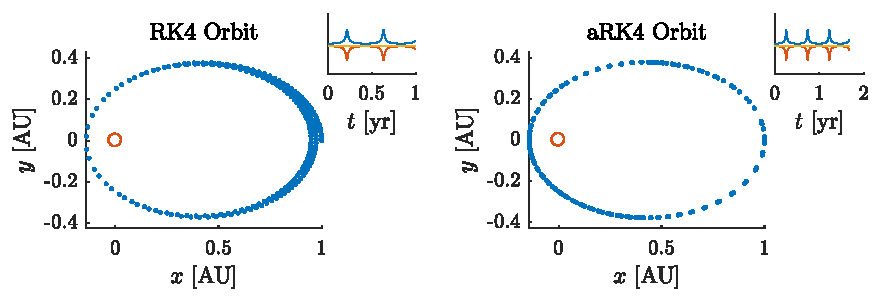
\includegraphics[width = \linewidth]{RK41pi.pdf}
		\caption{Same plot setup as before, but for an elliptical orbit}
		\label{fig:KeplerAdaptive2}
	\end{figure}
	
	Furthermore to see the adaptiveness in action, the step size $ \Delta t$ is plotted as a function of the radial distance:
	
	\begin{figure}[H]
		\centering
		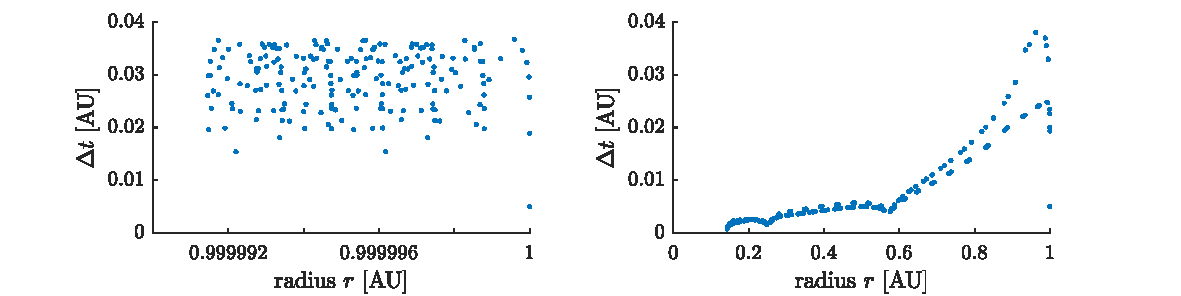
\includegraphics[width = \linewidth]{aRK4DT.pdf}
		\caption{Plots of the time step size $ \Delta t $, as a function of radial distance, for a circular (left) and elliptical (right) orbit.}
		\label{fig:KeplerAdaptiveDT}
	\end{figure}
	As seen in figure \ref{fig:KeplerAdaptive1}, both methods accurately simulate the circular orbit. However, with the same number of iterations, the adaptive method completes almost 6 full orbits, whilst the non-adaptive completes only one. This shows that the initial step size was small enough, that an increase in its size did not result in any significant errors. For the elliptical orbit, however, the non-adaptive method performs significantly worse than the adaptive one. The reason for this is seen in figure \ref{fig:KeplerAdaptiveDT}, where it is seen that the step size around the smallest radius is smaller than the initial value of $ \Delta t $. This suggests that for the non-adaptive method to produce accurate results, the step size should be reduced.
	
	The step sizes shown in figure \ref{fig:KeplerAdaptiveDT} shows the adaptiveness at work. In the circular orbit the size of the time step oscillates as the error oscillates around the upper bound set. For the elliptical orbit, the step size decreases as the radius decreases. This makes sense, as the velocity increases when the radius decreases, which necessitates a smaller time step, if the error bound is to be satisfied. In both cases the initial step size is well within the upper bound, and the size is quickly increased.
	
	
\end{document}

